\documentclass[12pt,fleqn]{article}\usepackage{../../common}
\begin{document}
Ders 1-15

Makaskirişler (Truss)

Bir makaşkiriş esneyebilen çubuklardan (bar) oluşur, bu çubuklar birbirine
bağlantı pimleri (pin joint) ile bağlıdır. Bağlantı pimi derken şunu
kastediyorum, çubukları esnetmek özellikle uzunluğu yönünde kuvvet gerektirir,
ama pim etrafında çubukları döndürmek efor gerektirmez.

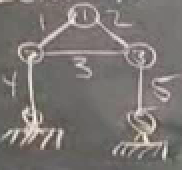
\includegraphics[width=10em]{compscieng_1_15_01.png}

Mesela resimdeki 3 no'lu çubuğu sağa ve sola esnetmek zor, ama o çubuğu
3 no'lu pim etrafında döndürmek kolay.

Bu derste iki boyutlu makaşkirişler incelenecek, daha önce iki boyutlu yay-kütle
sistemini incelediğimiz gibi; muhakkak üç boyutlu makaşkiriş sistemleri de var
ama iki boyut üzerinde ana başlıkları daha rahat olarak inceleyebiliriz.

Üstte görülen örnekte 5 tane çubuk 3 tane düğüm (nod, pim noktası) görüyorum.
Peki bilinmeyenler ne? Yani daha önceki yay-kütle problemindeki hesapladığımız
$u$ nedir? Çünkü $u$'dan $e$'ye oradan $w$'ya oradan da $f$'ye gitmek
istiyorum. İlk geçişi matris $A$ yapar, ikinciyi $C$, üçüncüyü $A^T$..
Bildiğimiz şeyler bunlar ama bu yapıyı önümüzdeki probleme göre oluşturmak
gerekiyor. Bahsettiğimiz matrislerin içini doldurmamız gerekiyor.

O zaman yapıyı tarif edelim. Mesela önce 1 no'lu düğüme bakalım, ona etki eden
kuvvetler nedir? İk boyuttayız demiştik, o zaman bir yatay bir de dikey kuvvet
olacak, en azından o düğüme etki eden tüm kuvvetler bu iki eksen bağlamında
incelenebilir. Bilinmeyeni $u$'yu bu fırsatla tanıştırıyorum, alttaki resimde
mesela ikinci düğümdeki yer değişimini yatay ve dikey bileşenlerine ayırarak
gösterebilirim,

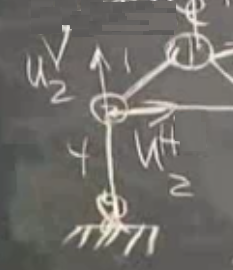
\includegraphics[width=8em]{compscieng_1_15_02.png}

Bileşenler yatay yönde $u_2^H$, dikey yönde $u_2^V$. Bu yer değişimlerini,
yatay, dikey her pim için yaparız, böylece, bir anlamda elimizdeki biinmeyen
değişken sayısı ikiye katlanmış oldu. Artı, eksi olabilen tek bir $u$ öğesi
yerine artık her düğüm için iki tane $u$ öğesi takip etmemiz gerekiyor.

Şimdi alttaki yere bağlı destek noktalarına bakalım; orada ne oluyor?  Bu
noktalarda ne sağa, ne sola, ne yukarı aşağı hareket var, çünkü oraları
sabitlendi. O zaman $u_4^H = u_4^V = 0 = u_5^H = u_5^V = 0$.  Toplam kaç tane
bilinmeyen var? Altı tane. 1,2,3 düğümleri için ikiser tane, sabitlenmiş
noktalarda yok, onlar biliniyor. Demek ki $A$ matrisim 5 x 6 boyutunda olacak.
Bu yapı bize 6 tane $u$, 5 tane $e$, 5 tane çubuk kuvveti, ve 6 tane denge
denklemi verecetir.




















[devam edecek]

\end{document}
